%%%%%%%%%%%%%%%%%%%%%%%%%%%%%%%%%%%%%%%%%
% Lachaise Assignment
% LaTeX Template
% Version 1.1(26/6/2018)
%
% This template originates from:
% http://www.LaTeXTemplates.com
%
% Authors:
% Marion Lachaise & François Févotte
% Vel (vel@LaTeXTemplates.com)
%
% License:
% CC BY-NC-SA 3.0 (http://creativecommons.org/licenses/by-nc-sa/3.0/)
% 
%%%%%%%%%%%%%%%%%%%%%%%%%%%%%%%%%%%%%%%%

%----------------------------------------------------------------------------------------
%	PACKAGES AND OTHER DOCUMENT CONFIGURATIONS
%----------------------------------------------------------------------------------------

\documentclass{article}

%%%%%%%%%%%%%%%%%%%%%%%%%%%%%%%%%%%%%%%%%
% Lachaise Assignment
% Structure Specification File
% Version 1.0 (26/6/2018)
%
% This template originates from:
% http://www.LaTeXTemplates.com
%
% Authors:
% Marion Lachaise & François Févotte
% Vel (vel@LaTeXTemplates.com)
%
% License:
% CC BY-NC-SA 3.0 (http://creativecommons.org/licenses/by-nc-sa/3.0/)
% 
%%%%%%%%%%%%%%%%%%%%%%%%%%%%%%%%%%%%%%%%%

%----------------------------------------------------------------------------------------
%	PACKAGES AND OTHER DOCUMENT CONFIGURATIONS
%----------------------------------------------------------------------------------------

\usepackage{amsmath,amsfonts,stmaryrd,amssymb,bbm,float,graphicx,enumerate,mathtools,listings,xcolor,color,esint,subfig,tikz,pgfplots,adjustbox,setspace,bm,minted,pdfpages,hyperref} % Math packages

\usepackage{enumerate} % Custom item numbers for enumerations

\usepackage[lined,boxed,vlined,ruled]{algorithm2e}
\SetKw{Continue}{continue}
\SetKw{Or}{or}
\SetKw{Until}{until}

\usepackage[framemethod=tikz]{mdframed} % Allows defining custom boxed/framed environments

\usepackage{listings} % File listings, with syntax highlighting
\lstset{
    basicstyle=\ttfamily, % Typeset listings in monospace font
}

\DeclarePairedDelimiter\ceil{\lceil}{\rceil}
\DeclarePairedDelimiter\floor{\lfloor}{\rfloor}

% Allow for the \begin{align} to go over the page
\allowdisplaybreaks

%----------------------------------------------------------------------------------------
%	DOCUMENT MARGINS
%----------------------------------------------------------------------------------------

\usepackage{geometry} % Required for adjusting page dimensions and margins

\geometry{
    paper=a4paper, % Paper size, change to letterpaper for US letter size
    top=2.5cm, % Top margin
    bottom=3cm, % Bottom margin
    left=2.5cm, % Left margin
    right=2.5cm, % Right margin
    headheight=14pt, % Header height
    footskip=1.5cm, % Space from the bottom margin to the baseline of the footer
    headsep=1.2cm, % Space from the top margin to the baseline of the header
    %showframe, % Uncomment to show how the type block is set on the page
}

%----------------------------------------------------------------------------------------
%	FONTS
%----------------------------------------------------------------------------------------

\usepackage[utf8]{inputenc} % Required for inputting international characters
\usepackage[T1]{fontenc} % Output font encoding for international characters

\usepackage{XCharter} % Use the XCharter fonts

%----------------------------------------------------------------------------------------
%	COMMAND LINE ENVIRONMENT
%----------------------------------------------------------------------------------------

% Usage:
% \begin{commandline}
%	\begin{verbatim}
%		$ ls
%		
%		Applications	Desktop	...
%	\end{verbatim}
% \end{commandline}

\mdfdefinestyle{commandline}{
    leftmargin=10pt,
    rightmargin=10pt,
    innerleftmargin=15pt,
    middlelinecolor=black!50!white,
    middlelinewidth=2pt,
    frametitlerule=false,
    backgroundcolor=black!5!white,
    frametitle={Command Line},
    frametitlefont={\normalfont\sffamily\color{white}\hspace{-1em}},
    frametitlebackgroundcolor=black!50!white,
    nobreak,
}

% Define a custom environment for command-line snapshots
\newenvironment{commandline}{
    \medskip
    \begin{mdframed}[style=commandline]
        }{
    \end{mdframed}
    \medskip
}

%----------------------------------------------------------------------------------------
%	FILE CONTENTS ENVIRONMENT
%----------------------------------------------------------------------------------------

% Usage:
% \begin{file}[optional filename, defaults to "File"]
%	File contents, for example, with a listings environment
% \end{file}

\mdfdefinestyle{file}{
    innertopmargin=1.6\baselineskip,
    innerbottommargin=0.8\baselineskip,
    topline=false, bottomline=false,
    leftline=false, rightline=false,
    leftmargin=2cm,
    rightmargin=2cm,
    singleextra={%
            \draw[fill=black!10!white](P)++(0,-1.2em)rectangle(P-|O);
            \node[anchor=north west]
            at(P-|O){\ttfamily\mdfilename};
            %
            \def\l{3em}
            \draw(O-|P)++(-\l,0)--++(\l,\l)--(P)--(P-|O)--(O)--cycle;
            \draw(O-|P)++(-\l,0)--++(0,\l)--++(\l,0);
        },
    nobreak,
}

% Define a custom environment for file contents
\newenvironment{file}[1][File]{ % Set the default filename to "File"
    \medskip
    \newcommand{\mdfilename}{#1}
    \begin{mdframed}[style=file]
        }{
    \end{mdframed}
    \medskip
}

%----------------------------------------------------------------------------------------
%	NUMBERED QUESTIONS ENVIRONMENT
%----------------------------------------------------------------------------------------

% Usage:
% \begin{question}[optional title]
%	Question contents
% \end{question}

\mdfdefinestyle{question}{
    innertopmargin=1.2\baselineskip,
    innerbottommargin=0.8\baselineskip,
    roundcorner=5pt,
    nobreak,
    singleextra={%
            \draw(P-|O)node[xshift=1em,anchor=west,fill=white,draw,rounded corners=5pt]{%
                Question \theQuestion\questionTitle};
        },
}

\newcounter{Question} % Stores the current question number that gets iterated with each new question

% Define a custom environment for numbered questions
\newenvironment{question}[1][\unskip]{
    \bigskip
    \stepcounter{Question}
    \newcommand{\questionTitle}{~#1}
    \begin{mdframed}[style=question]
        }{
    \end{mdframed}
    \medskip
}

%----------------------------------------------------------------------------------------
%	WARNING TEXT ENVIRONMENT
%----------------------------------------------------------------------------------------

% Usage:
% \begin{warn}[optional title, defaults to "Warning:"]
%	Contents
% \end{warn}

\mdfdefinestyle{warning}{
    topline=false, bottomline=false,
    leftline=false, rightline=false,
    nobreak,
    singleextra={%
            \draw(P-|O)++(-0.5em,0)node(tmp1){};
            \draw(P-|O)++(0.5em,0)node(tmp2){};
            \fill[black,rotate around={45:(P-|O)}](tmp1)rectangle(tmp2);
            \node at(P-|O){\color{white}\scriptsize\bf !};
            \draw[very thick](P-|O)++(0,-1em)--(O);%--(O-|P);
        }
}

% Define a custom environment for warning text
\newenvironment{warn}[1][Warning:]{ % Set the default warning to "Warning:"
    \medskip
    \begin{mdframed}[style=warning]
        \noindent{\textbf{#1}}
        }{
    \end{mdframed}
}

%----------------------------------------------------------------------------------------
%	INFORMATION ENVIRONMENT
%----------------------------------------------------------------------------------------

% Usage:
% \begin{info}[optional title, defaults to "Info:"]
% 	contents
% 	\end{info}

\mdfdefinestyle{info}{%
topline=false, bottomline=false,
leftline=false, rightline=false,
nobreak,
singleextra={%
\fill[black](P-|O)circle[radius=0.4em];
\node at(P-|O){\color{white}\scriptsize\bf i};
\draw[very thick](P-|O)++(0,-0.8em)--(O);%--(O-|P);
}
}

% Define a custom environment for information
\newenvironment{info}[1][Info:]{ % Set the default title to "Info:"
    \medskip
    \begin{mdframed}[style=info]
        \noindent{\textbf{#1}}
        }{
    \end{mdframed}
}

\pgfplotsset{compat=1.12}
\usepgfplotslibrary{fillbetween}
\DeclareMathOperator{\sech}{sech}
\DeclareMathOperator{\arcsech}{arcsech}
\DeclareMathOperator{\arcoth}{arcoth}
\DeclareMathOperator{\arctanh}{tanh^{-1}}
\renewcommand{\baselinestretch}{1.25}
\newcommand{\bin}{{\sf Bin}}
\newcommand{\G}{{\sf G}}
\newcommand{\Hyp}{{\sf Hyp}}
\newcommand{\Ber}{{\sf Ber}}
\newcommand{\Po}{{\sf Po}}
\newcommand{\Poi}{{\sf Poi}}
\newcommand{\ex}{{\sf Exp}}
\newcommand{\Nor}{{\sf N}}
\newcommand{\gam}{{\sf Gam}}
\newcommand{\Em}{\mathbb E}
\newcommand{\Pm}{\mathbb P}
\newcommand{\R}{\mathbb R}
\newcommand{\Cm}{\mathbb C}
\newcommand{\B}{\cal B}
\newcommand{\F}{\mathbb F}
\newcommand{\N}{\mathbb N}
\newcommand{\Z}{\mathbb Z}
\newcommand{\Q}{\mathbb Q}
\newcommand{\Comp}{\mathbb C}
\newcommand{\e}{\mbox{e}}
\newcommand{\Var}{\mbox{Var}}
\newcommand{\cov}{\mbox{Cov}}
\newcommand{\ds}{\displaystyle}
\newcommand{\subvect}[1]{\mbox{\small \boldmath #1}}
%\newcommand{\vect}[1]{\mbox{\boldmath $#1$}}
\newcommand{\vect}[1]{\boldsymbol #1}
\newcommand{\norm}[1]{\left\lVert#1\right\rVert}
\newcommand*\VF[1]{\mathbf{#1}}
\newcommand*\dif{\mathop{}\!\mathrm{d}}
\setlength{\jot}{7pt}
\definecolor{lbcolor}{rgb}{0.95,0.95,0.95}

\title{COMP4702: 2021 Final Exam} % Title of the assignment

\author{Michael Ciccotosto-Camp\\ \texttt{s4430291}} % Author name and email address

\date{University of Queensland --- \today}
\begin{document}

\maketitle % Print the title

\section*{Data Edits and Visualizations}

% \begin{itemize}
%     \item What changes where made to the dataset. Were rows/columns removed or edited? Why?
%     \item What any standardization/normalization performed?
%     \item Does the data look easy to separate when projected onto a lower dimension using PCA,TSNE, etc? How might this influence which model we use?
%     \item Graph the covariances between the data.
% \end{itemize}

To start rows that contained Nan values where removed from the data set so that all the features could be utilized for prediction. It was decided that we should try and regress of the "ViolentCrimesPerPop" since most other measurements can easily be accquired for by a national survey, but we cannot as easily survey the number of crimes that happen within a community. The "communityname" row was removed since it was mostly unique to many of the rows and therefore would not give much on the number of crimes. Next the columns were standardised and columns with the lowest 80 percent of variance where removed since columns with low variance will likely not provide much information. Some statistics for the data is shown below in table form.

\begin{table}[h!]
    \centering
    \begin{tabular}{lrrrrrrrr}
        \hline
                            & count & mean      & std      & min & 25\% & 50\% & 75\% & max \\
        \hline
        state               & 1993  & 28.6939   & 16.3951  & 1   & 12   & 34   & 42   & 56  \\
        fold                & 1993  & 5.49624   & 2.87265  & 1   & 3    & 5    & 8    & 10  \\
        racepctblack        & 1993  & 0.179709  & 0.25348  & 0   & 0.02 & 0.06 & 0.23 & 1   \\
        racePctWhite        & 1993  & 0.753643  & 0.244079 & 0   & 0.63 & 0.85 & 0.94 & 1   \\
        racePctHisp         & 1993  & 0.144009  & 0.232549 & 0   & 0.01 & 0.04 & 0.16 & 1   \\
        pctUrban            & 1993  & 0.696116  & 0.44487  & 0   & 0    & 1    & 1    & 1   \\
        PctIlleg            & 1993  & 0.25005   & 0.229991 & 0   & 0.09 & 0.17 & 0.32 & 1   \\
        PctRecentImmig      & 1993  & 0.18142   & 0.235837 & 0   & 0.03 & 0.09 & 0.23 & 1   \\
        PctRecImmig5        & 1993  & 0.182183  & 0.236379 & 0   & 0.03 & 0.08 & 0.23 & 1   \\
        PctRecImmig8        & 1993  & 0.184827  & 0.236787 & 0   & 0.03 & 0.09 & 0.23 & 1   \\
        PctRecImmig10       & 1993  & 0.18293   & 0.23487  & 0   & 0.03 & 0.09 & 0.23 & 1   \\
        MedNumBR            & 1993  & 0.314601  & 0.255212 & 0   & 0    & 0.5  & 0.5  & 1   \\
        MedYrHousBuilt      & 1993  & 0.494099  & 0.232499 & 0   & 0.35 & 0.52 & 0.67 & 1   \\
        PctHousNoPhone      & 1993  & 0.264541  & 0.242892 & 0   & 0.06 & 0.19 & 0.42 & 1   \\
        OwnOccMedVal        & 1993  & 0.263527  & 0.231594 & 0   & 0.09 & 0.17 & 0.39 & 1   \\
        OwnOccHiQuart       & 1993  & 0.268986  & 0.235303 & 0   & 0.09 & 0.18 & 0.38 & 1   \\
        RentHighQ           & 1993  & 0.422985  & 0.248346 & 0   & 0.22 & 0.37 & 0.59 & 1   \\
        PctForeignBorn      & 1993  & 0.2156    & 0.231182 & 0   & 0.06 & 0.13 & 0.28 & 1   \\
        LemasPctOfficDrugUn & 1993  & 0.0939388 & 0.240335 & 0   & 0    & 0    & 0    & 1   \\
        ViolentCrimesPerPop & 1993  & 0.237998  & 0.233042 & 0   & 0.07 & 0.15 & 0.33 & 1   \\
        \hline
    \end{tabular}
\end{table}

Boxplots where also employeed to give a better visualizations on the spread of each feature.

\begin{figure}[H]
    \centering
    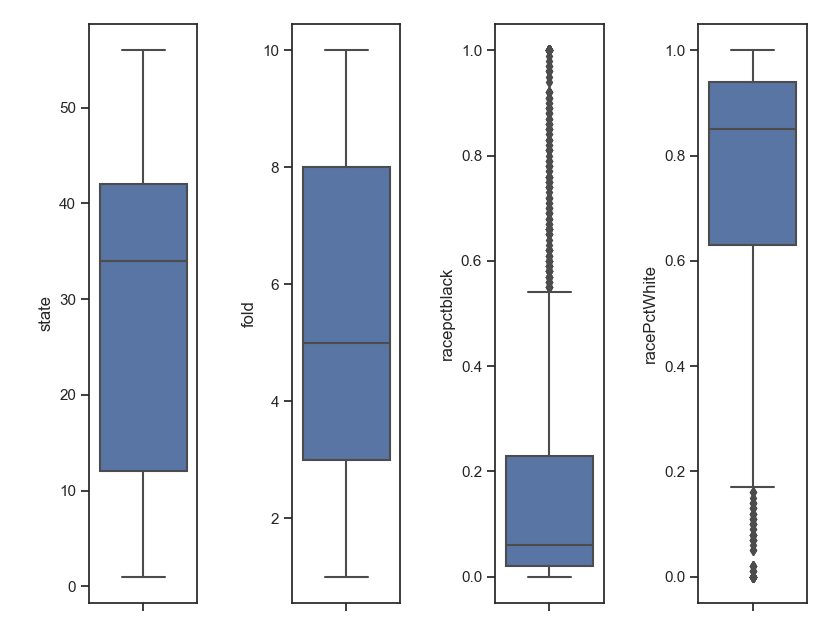
\includegraphics[scale=0.5]{bp_1.png}
\end{figure}


\begin{figure}[H]
    \centering
    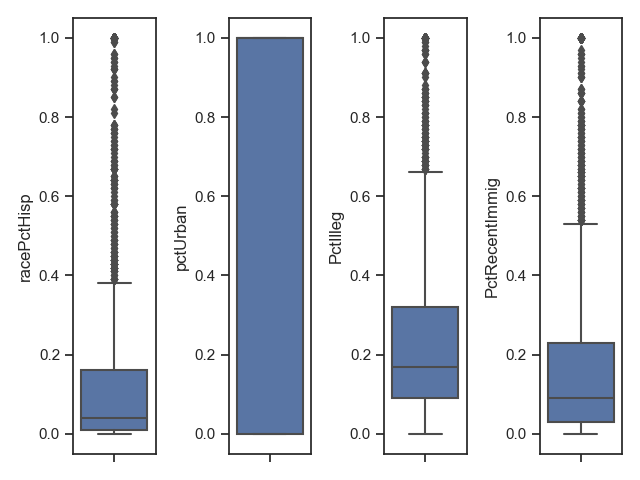
\includegraphics[scale=0.5]{bp_2.png}
\end{figure}

\begin{figure}[H]
    \centering
    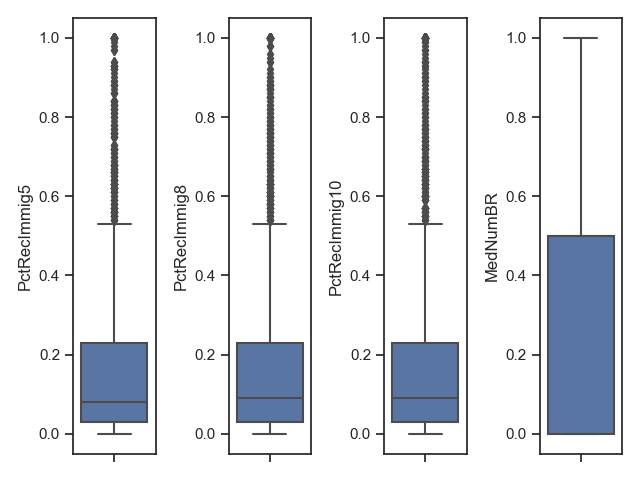
\includegraphics[scale=0.5]{bp_3.png}
\end{figure}

\begin{figure}[H]
    \centering
    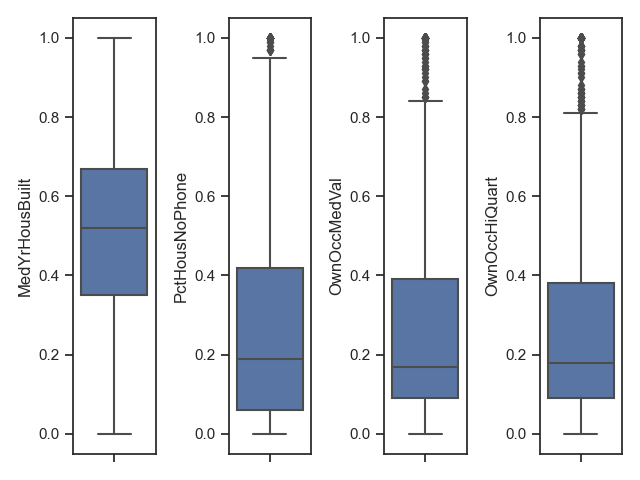
\includegraphics[scale=0.5]{bp_4.png}
\end{figure}

\begin{figure}[H]
    \centering
    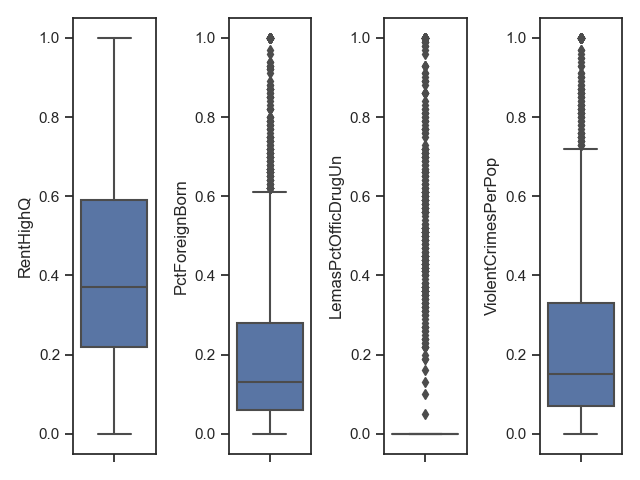
\includegraphics[scale=0.5]{bp_5.png}
\end{figure}

A SCREE graph and covariance matrix was also produced for this data set.

\begin{figure}[H]
    \centering
    
\includegraphics[scale=0.5]{SCREE.png}
    \caption{SCREE graph}
\end{figure}

\begin{figure}[H]
    \centering
    
\includegraphics[scale=0.4]{cov_mat.png}
    \caption{Covariance Matrix}
\end{figure}

One thing to notice is that the vast majority of importance weighting in the spree graph resides in the first 5 principal components. This suggests that the data undergo dimensionality reduction without too much feature information loss. This is supported by the fact that there are a number of correlations depicted in the covariance matrix. A number of dimensionality reduction techniques were used project the data onto a 2-dimensional to see how well they separate out the data. Each feature was standardized before hand so that the dimensionality reduction techniques so that no feature had a information retention weighting. The techniques used were PCA, TSNE and Isomapping. The results are presented below.

\begin{figure}[H]
    \centering
    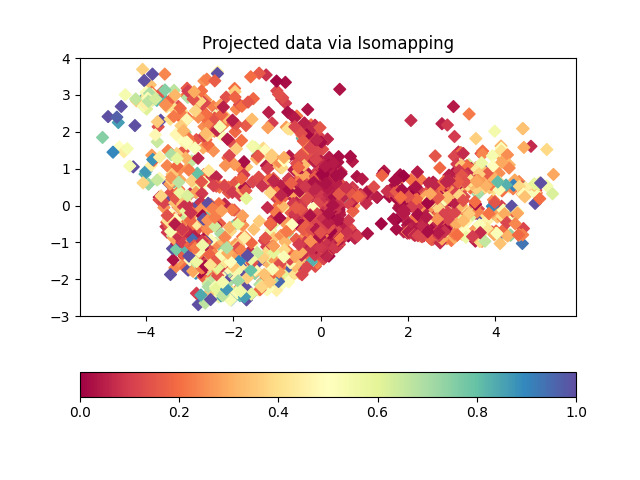
\includegraphics[scale=0.7]{ISO_proj.png}
\end{figure}

\begin{figure}[H]
    \centering
    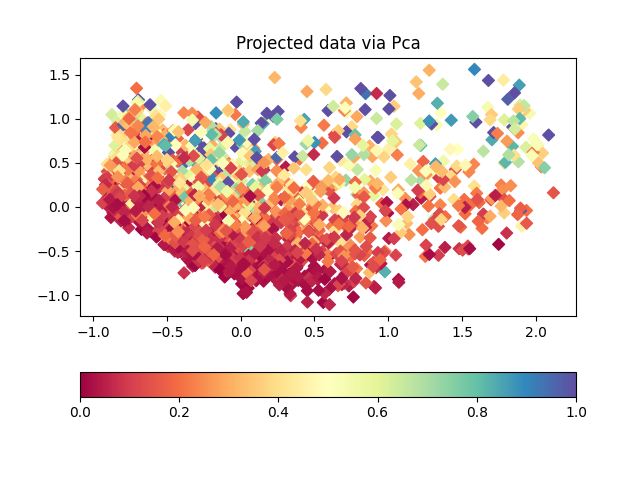
\includegraphics[scale=0.7]{PCA_proj.png}
\end{figure}

\begin{figure}[H]
    \centering
    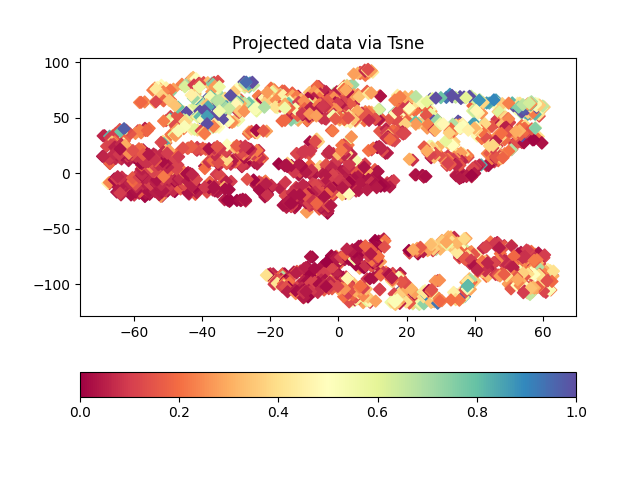
\includegraphics[scale=0.7]{TSNE_proj.png}
\end{figure}

PCA was chosen to be the preferred method for dimensionality reduction since it seemed to organise the inputs much nice than the other two methods with crime rate going up as the first principal component increased.

\section*{Gaussian Processes Regression}

An GPR model was chosen since GPRs are designed to perform classification tasks on continuous inputs. The RBF kernel was used as the kernel parameter since, when looking at the PCA projection, predictions could be made by looking at surrounding points. Transforming the data using PCA where the first $15$ components are retained seemed to provided the best performance. A grid search was used to find the best parameters for the length parameter ($\alpha$). To do this, numerous GPR model's were trained with different values for $\alpha$ and the performance of each model was measured by averaging the mean square error of a 5-fold cross validation partition. The results of the grid search are shown below. The length parameter of the kernel was found using a gridsearch. The results of the gridsearch are shown below.

\begin{figure}[H]
    \centering
    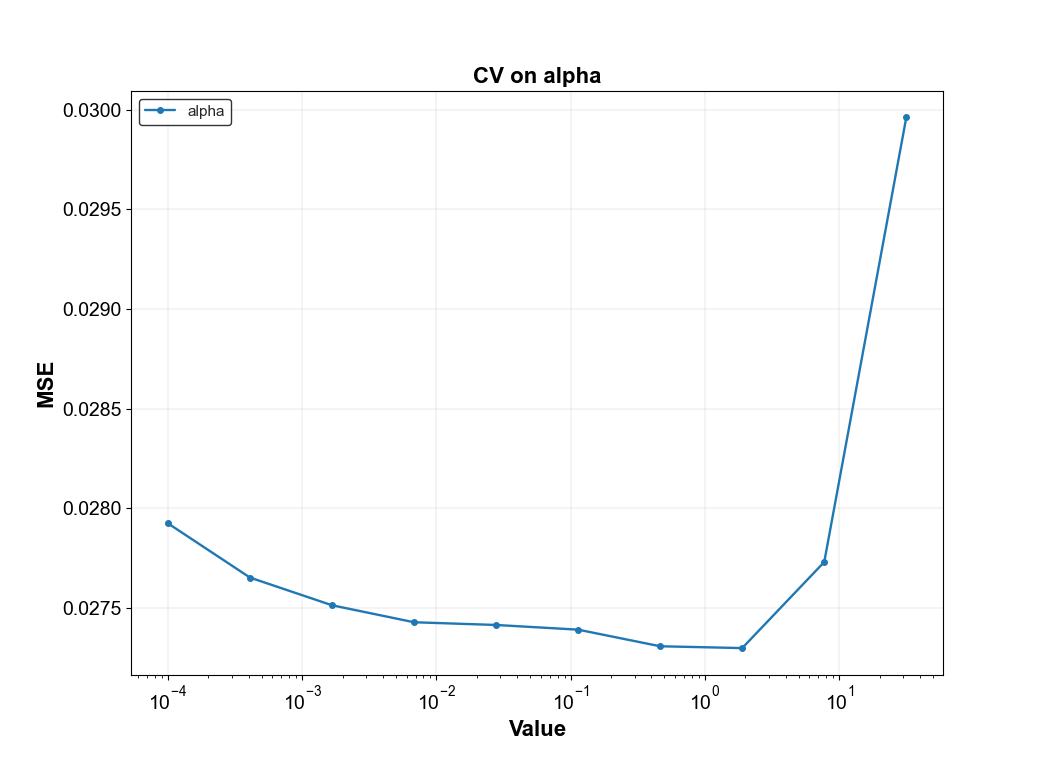
\includegraphics[scale=0.5]{gpr_mse.png}
\end{figure}

Hence $\alpha = 2$ was used for model training. The training and testing MSE on a typical runs with this set up was $0.0173388$ and $0.0200241$ respectively, where $1/5$ of the data is retained for testing. A visualization of model predictions is shown below for a typical run when $1/5$ of the dataset is reversed for testing. The data is projected onto a 2-dimensional plane via PCA.

\begin{figure}[H]
    \centering
    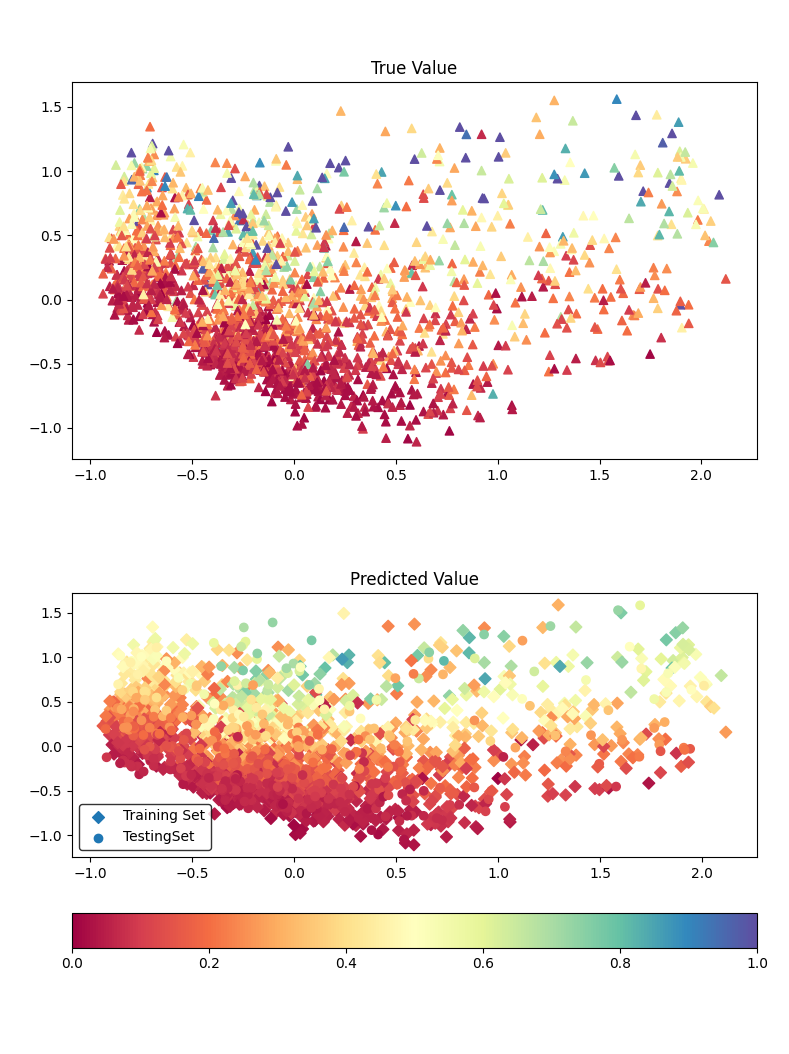
\includegraphics[scale=0.5]{true_vs_pred_gpr.png}
\end{figure}

We can see that while GPR does a good job of caputuring big-picture patterns, it suffers from smoothing over the predictions too much.

% \begin{itemize}
%     \item What model was chosen? Explain why the selected model is suitable for the task at hand (eg its a good idea use SVC if a classification problem is given to us and all the inputs are continuous).
%     \item What parameters were selected? Were they adjusted/how?
% \end{itemize}

\section*{Random Forest Regressor}

A random forest model was also used since they are a very versatile model and have an automated feature selection mechanism to seek which features may be most pertinent to predicting "ViolentCrimesPerPop". No transformation to the data was made when training the Random Forest Regressor (RFR). A grid search was used to find the best parameters for the max depth and the max features. To do this, numerous GPR model's were trained with different values for max depth and the max features and the performance of each model was measured by averaging the mean square error of a 5-fold cross validation partition. The results of the grid search are shown below. The results of the gridsearch are shown below.

\begin{figure}[H]
    \centering
    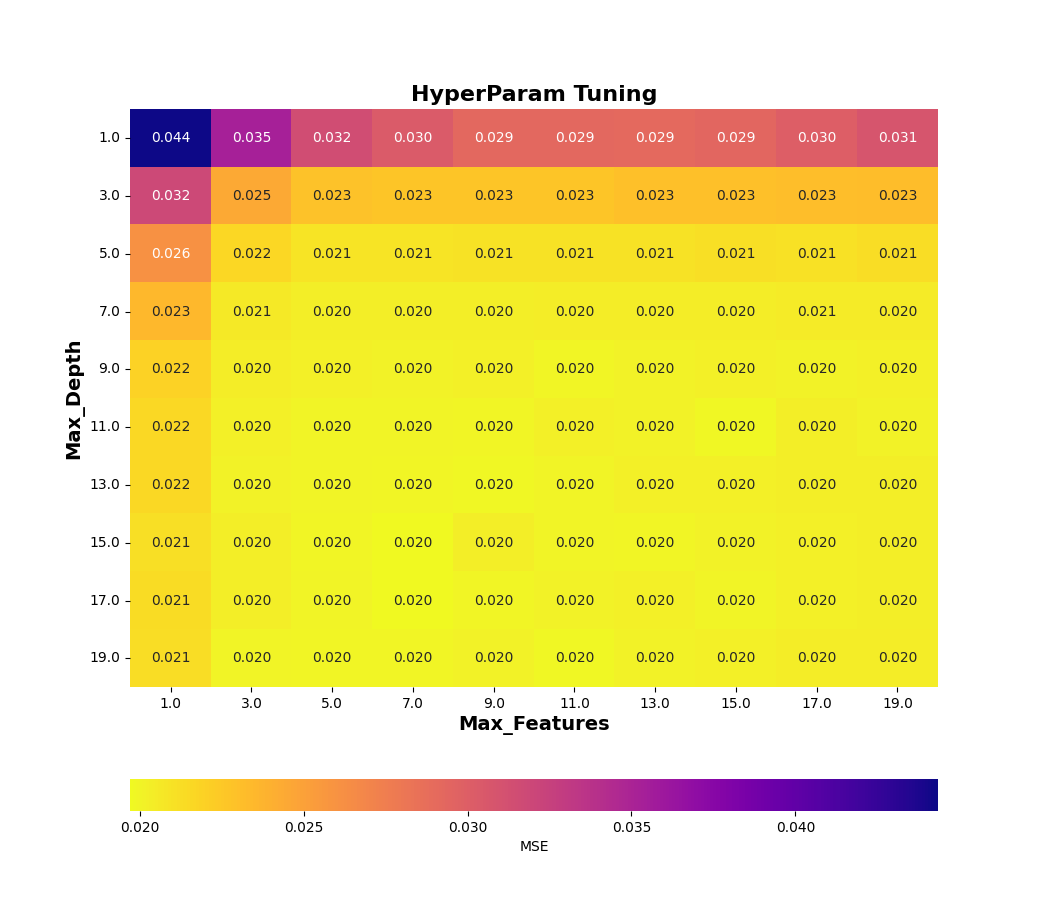
\includegraphics[scale=0.5]{rg_param_tune.png}
\end{figure}

Hence max depth was set to $11$ and max features was set to $9$ was used for model training. The training and testing MSE on 10 typical runs with this set up is shown in the below table, where $1/5$ of the data is retained for testing.

\begin{table}[h!]
    \centering
    \begin{tabular}{rrr}
        \hline
        Repetition & Train MSE  & Test MSE  \\
        \hline
        1          & 0.00278352 & 0.020284  \\
        2          & 0.00279283 & 0.0204085 \\
        3          & 0.00283465 & 0.0202092 \\
        4          & 0.00278479 & 0.0204838 \\
        5          & 0.00284724 & 0.0203834 \\
        6          & 0.00283097 & 0.02055   \\
        7          & 0.0027767  & 0.0203615 \\
        8          & 0.00287339 & 0.0202939 \\
        9          & 0.00281724 & 0.0202996 \\
        10         & 0.00280879 & 0.0202641 \\
        \hline
    \end{tabular}
\end{table}

A visualization of model predictions is shown below for a typical run when $1/5$ of the dataset is reversed for testing. The data is projected onto a 2-dimensional plane via PCA.

\begin{figure}[H]
    \centering
    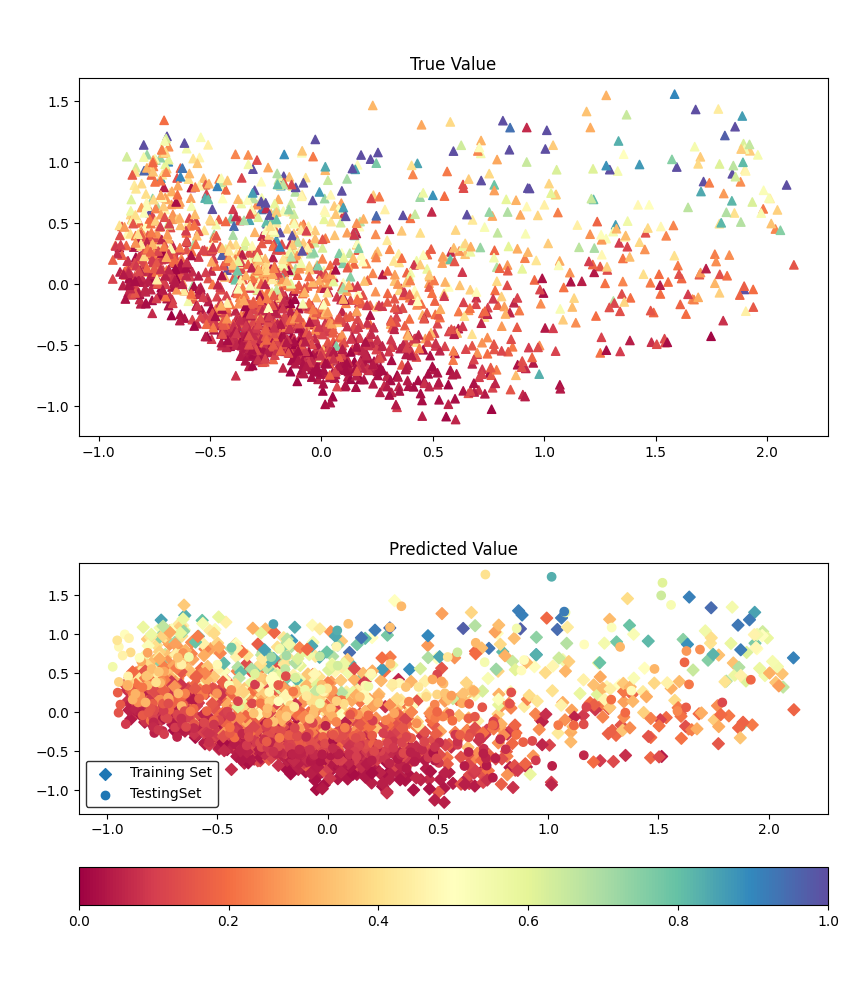
\includegraphics[scale=0.5]{true_vs_pred_rf.png}
\end{figure}

\section*{Neural Network Model}

A neural network model was also used since, although PCA provides a good separation of classes in lower dimensions, there is still small amount of overlap causing models to smooth over results too much. The complexity of a neural network architecture may mean it could learn a non-trivial way to separate and classify points. To this end, an initial neural network architecture of a single hidden layer with relu activation and a single output with a sigmoid activation function was devised. The 7-layer hidden layer adds extra complexity to the model to assist in learning highly non-trivial and non-linear functions which one can also think of as also providing some sort of in-built dimensionality reduction. Relu activation functions were used for efficiently and are well known for generally providing good performance. An Adam optimizer was used as it combines RMSProp with standard momentum meaning it generally has better learning rate adaptation than most other optimizers such as Adagrad, RMSProp and AdaDelta. Mean Square Error was used as the loss function as it minimizes the average squared distances between the target output and true value and is incredibly simple to optimize. A grid search over the learning rates was done to determine which learning rates was optimal for model training. The performance of each learning rates was measured by averaging the accuracy of a 5-fold cross validation partition. The model accuracies using different learning rates and an epoch of 50 is graphed below.

\begin{figure}[H]
    \centering
    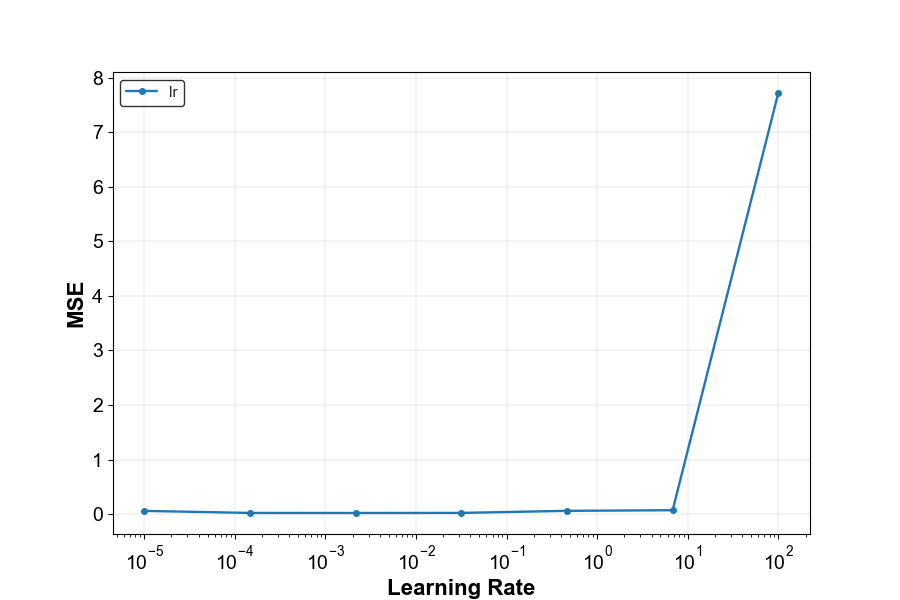
\includegraphics[scale=0.5]{nn_lr_tune.png}
\end{figure}

From the graph learning rates between $10^{-4}$ and $10^{-2}$ provided the best results and a learning rate of $10^{-3}$ was chosen for the remainder of experimentation. The validation and training loss was graphed over the number of epochs to see were overfitting may occur.

\begin{figure}[H]
    \centering
    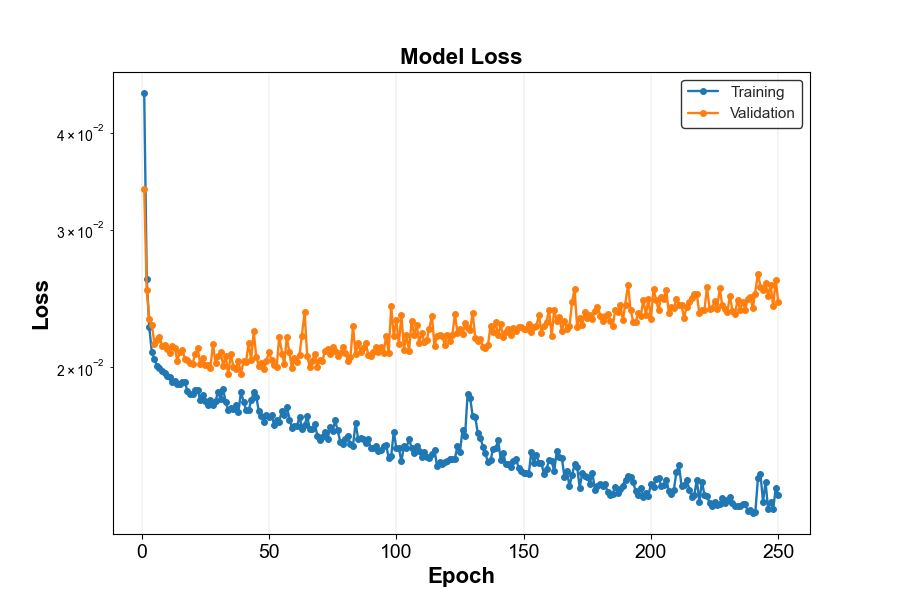
\includegraphics[scale=0.5]{epoch_tune.png}
\end{figure}

As we can see, training the model beyond 40 epochs is likely going to overfit our model (since the training loss seems to plateau and slightly increase beyond this value). Thus, the model was only trained with 40 epochs for the remainder of experimentation. A visualization of model predictions is shown below for a typical run when $1/5$ of the dataset is reversed for testing. The data is projected onto a 2-dimensional plane via PCA.

\begin{figure}[H]
    \centering
    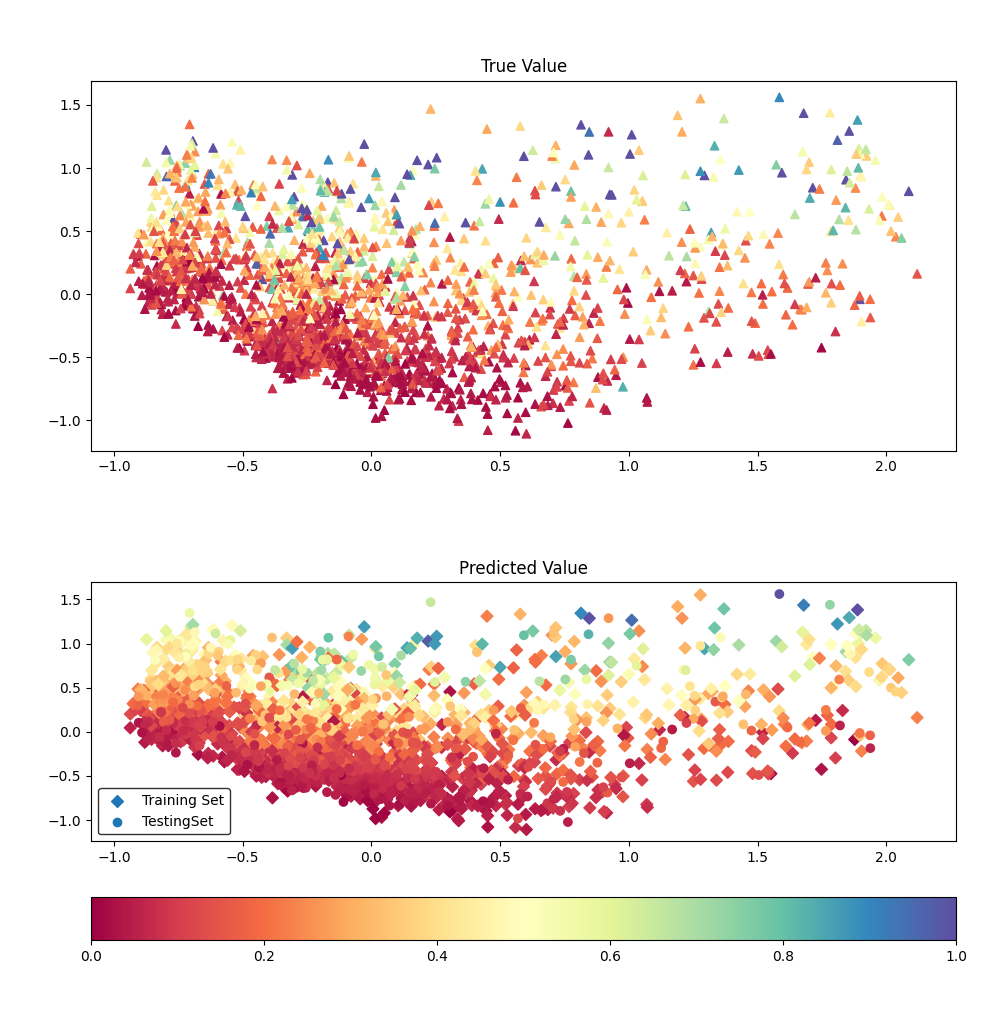
\includegraphics[scale=0.5]{true_vs_pred_nn.png}
\end{figure}

A visualization of model predictions is shown below for a typical run when $1/5$ of the dataset is reversed for testing. The data is projected onto a 2-dimensional plane via PCA.

\begin{table}[h!]
    \centering
    \begin{tabular}{rrr}
        \hline
        Repetition & Train MSE & Test MSE  \\
        \hline
        1          & 0.0687823 & 0.0789803 \\
        2          & 0.065448  & 0.0725585 \\
        3          & 0.0644822 & 0.0679641 \\
        4          & 0.0625274 & 0.069237  \\
        5          & 0.0631095 & 0.0688372 \\
        6          & 0.062796  & 0.0689889 \\
        7          & 0.0625975 & 0.0673013 \\
        8          & 0.0621537 & 0.067493  \\
        9          & 0.0620761 & 0.0659171 \\
        10         & 0.062894  & 0.0675226 \\
        \hline
    \end{tabular}
\end{table}


\section*{Future Improvements}

Most of the parameters were tuned using a brute force grid search method. In future, it would perhaps be better to instead employ a bayesian hyperparameter optimizer to cut down on computation and narrow in on a better parameter value faster.

% \section*{Results}

% \begin{itemize}
%     \item For a classification problem, graph out a confusion matrix. How might the data projects onto lower dimensions explain confusion between certain classes. If two classes to closer together when projected onto a lower dimension, then there is a good chance that the model may mistake them.
%     \item Graph how the true outputs compare to the predicted outputs.
%     \item What other improvements to the model could be made if more time was allowed?
% \end{itemize}

\end{document}